% !TeX spellcheck = en_US
\section{Race Detection by Mining Locking Rules}
\label{sec_technique}
To address the above challenges, we propose three key techniques. For {\em C1}, 
we propose an {\em alias-aware rule mining method} to automatically deduce 
locking rules. For {\em C2}, we propose a {\em lock-usage analysis} to filter 
out false data races by validating concurrency of code paths. For {\em C3}, we 
propose a pattern-based estimation to extract harmful races that can trigger 
memory or logical bugs such as null-pointer dereference and data inconsistency. 
We introduce them as follows:

\subsection{Alias-Aware Rule Mining Method}
\label{subsec_rule_mining}
The relationship between variables and locks are not well documented in OS 
kernels, but it can be inferred from the kernel code. Specifically, a data 
structure field is often protected by the lock stored in the same data 
structure. And thus if a data structure field is accessed after acquiring a 
lock existing in the same data structure in most cases, the variable is likely 
to be protected by the lock. Whether a data structure field and the protecting 
lock exist in the same data structure can be determined though an alias 
graph~\cite{Li:ASPLOS22, Kastrinis:CC18} by finding their common ancestor. 
Based on this insight, we propose an {\em alias-aware rule mining method} to 
deduce locking rules automatically. Moreover, with benefits from precise 
field-sensitive alias relationships of alias graph, our alias-aware rule mining 
method can find data structure filed and its protecting lock effectively.

\PP{Alias Graph.} It is an important data structure to infer relationships 
between data structure field and its protecting lock in our analysis, so we 
introduce it and its update first. 

An alias graph is a 2-tuple $\mathit{G = \left<N, E\right>}$, where 
$\mathit{N}$ is a set of nodes, and each node $\mathit{n}$ represents an alias 
set that points to one abstract object. $\mathit{E}$ is a set of labeled edges. 
Each edge is labeled with a data structure field or a dereference operator 
``$\mathit{*}$'', which represents how an abstract object is accessed.

An alias graph is updated by handling four types of instructions that  
change alias relationships: MOVE($\mathit{v_1 = v_2}$), STORE ($\mathit{*v_2 = 
v_1}$), LOAD ($\mathit{v_1 = *v_2}$) and GEP ({$\mathit{v_1 = \&v_1->f}$}). We 
exploit {$\mathit{n_x}$} to represent the node whose representing alias set 
includes $\mathit{v_x}$, and introduce how the four types of instructions 
update alias graphs. For a MOVE operation, $\mathit{v_1}$ is moved from 
$\mathit{n_1}$ to $\mathit{n_2}$. After this operation, $\mathit{v_1}$ and  
$\mathit{v_2}$ are represented by the same node, which indicates they become 
aliases. For a STORE operation, the existing outgoing edge from $\mathit{n_2}$ 
is dropped first, and then a new edge labeled with $\mathit{*}$ from 
$\mathit{n_2}$ to $\mathit{n_1}$ is inserted. After this operation, 
$\mathit{v_1}$ and $\mathit{*v_2}$ are represented by the same node, which 
indicates they become aliases. For a LOAD operation, the analysis first finds 
the destination node of the edge that comes from $\mathit{n_2}$ and is labeled 
with $\mathit{*}$, and then move $\mathit{v_1}$ to the destination node. And 
after this operation, $\mathit{v_1}$ and $\mathit{*v_2}$ are represented by the 
same node, which indicates they become aliases. GEP operation is similar to 
LOAD, expect that the edge is labeled with a data structure field $\mathit{f}$, 
instead of a dereference operator $\mathit{*}$.

\begin{figure}[htbp]
	\centering
	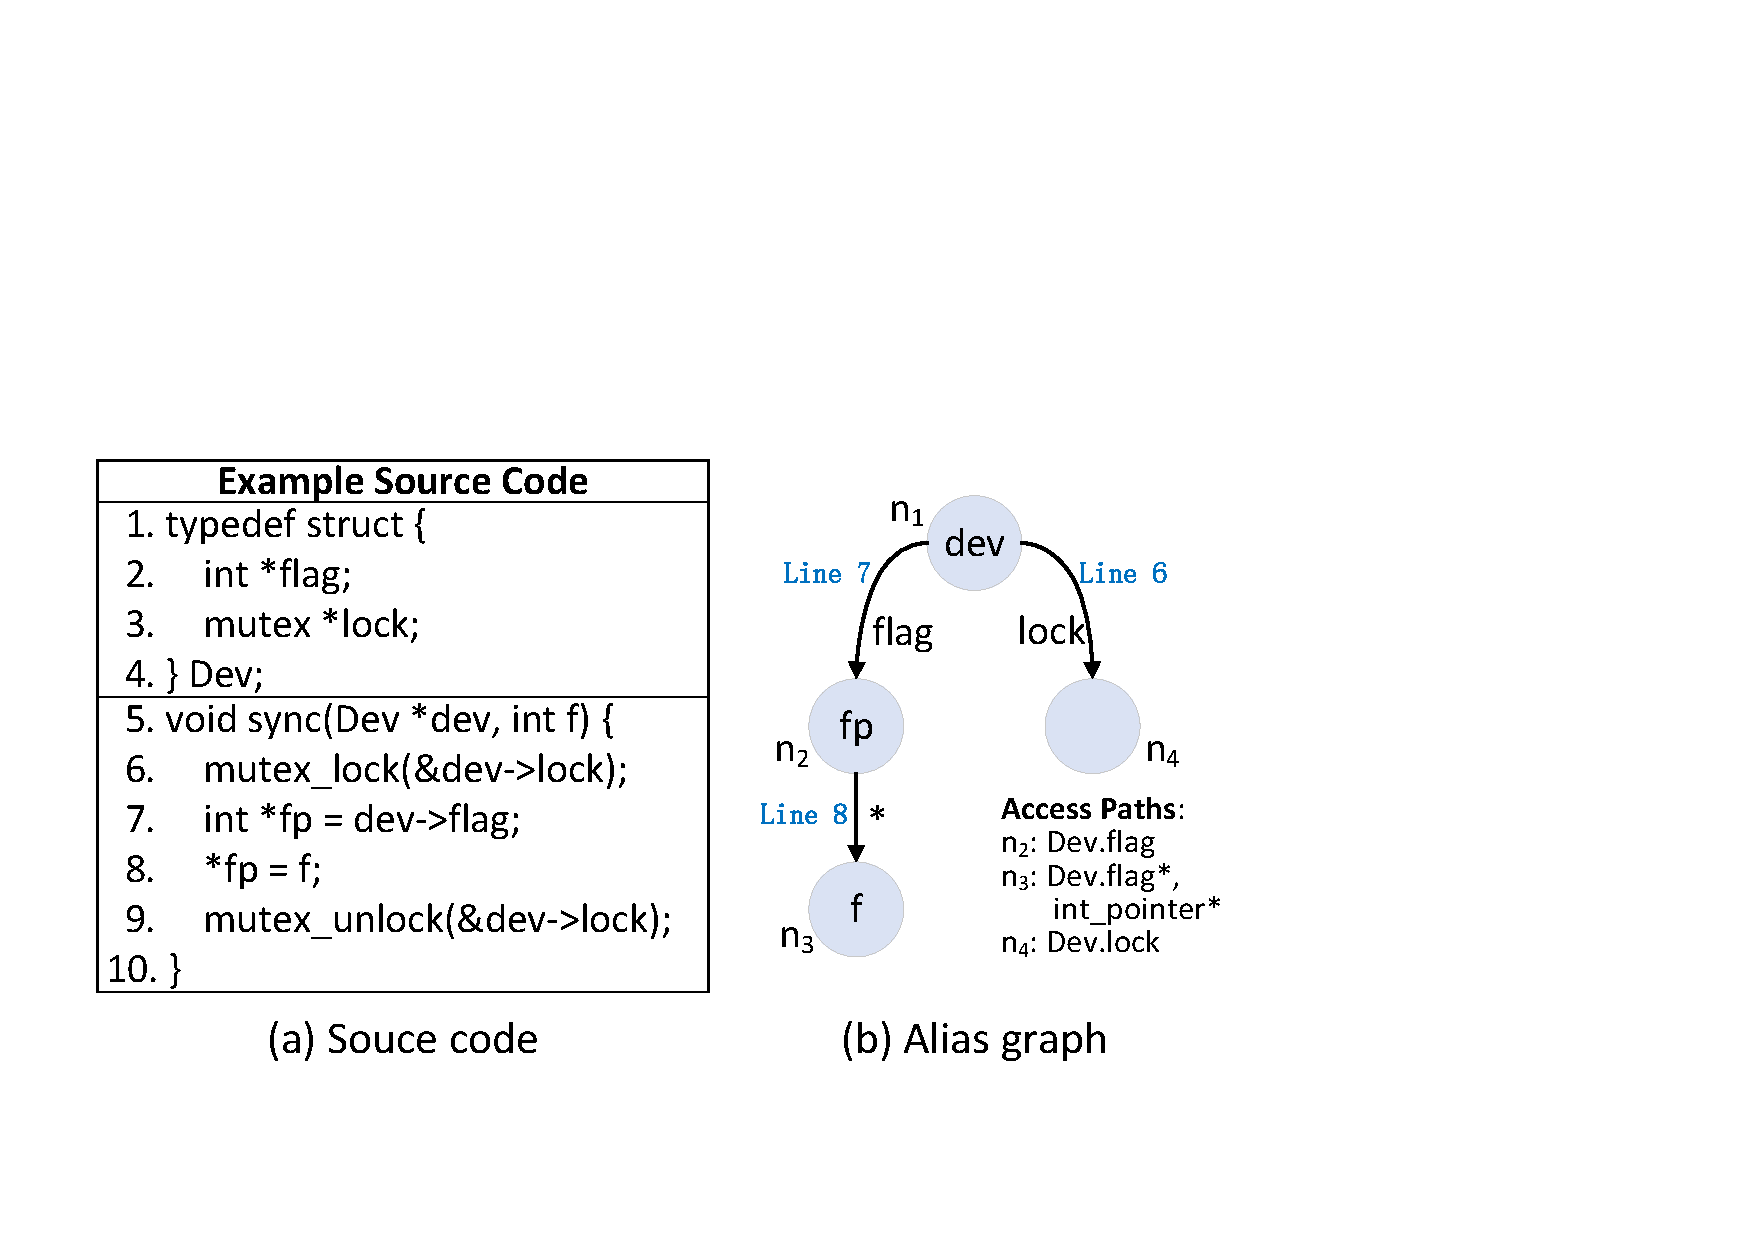
\includegraphics[width=0.9\linewidth]{figures/fig_alias_graph_demo.pdf}
	\figcaption{Example of alias graph.}
	\label{fig_alias_graph_demo}
\end{figure}

\noindent{\textbf{\em Example.}} Figure~\ref{fig_alias_graph_demo} shows a 
piece of driver-like source code and its alias graph. In this example, after an 
GEP (\&dev->lock) operation at Line 6, an edge labeled with {\tt lock} from 
node $\mathit{n_1}$ to node $\mathit{n_4}$ is inserted. Similarly, an edge 
labeled with {\tt flag} from node $\mathit{n_1}$ to node $\mathit{n_2}$ is 
inserted after Line 7. At last, an edge labeled with a dereference operator 
($\mathit{*}$) is inserted after the STORE (*fp = f) operation at Line 8. In 
this example, {\tt \&dev->flag} is represented by node $\mathit{n_2}$, and {\tt 
\&dev->lock} is represented by node $\mathit{n_4}$. The two nodes have a common 
ancestor $\mathit{n_1}$, and thus the accessed data structure field {\tt 
\&dev->flag} and the protecting lock {\tt \&dev->lock} can be inferred to exist 
in the same data structure (namely {\tt Dev}).